\monster{\hypertarget{malboro}{Malboro}}{7}{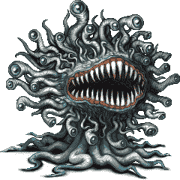
\includegraphics[width=0.21\textwidth]{./art/monsters/malboro.png}}
{
 PV: & \hfill 100 & PM: & \hfill 100 \\
 FUE: & \hfill 2 & DEF: & \hfill 4 \\
 MAG: & \hfill 5 & RES: & \hfill 7 \\
 AGI: & \hfill 2 & Tamaño: & \hfill G\\
}
{
 \textbf{Tentáculo}: 2d de daño \hfill \textbf{Botín:} 1000 Gil \\
 \textbf{Inmune}: \hyperlink{status}{Todos los Estados Alterados} \hfill \textbf{Debilidad}:\fire 
 
 \mtech{Mal Aliento}{20}{1t}{3u (frente)}{Tú}{
 Todos los enemigos en el área de efecto hacen una tirada con DC 8. Si fallan, quedan \hyperlink{status}{Dormidos},   \hyperlink{status}{Envenenados}, en \hyperlink{status}{Silencio} y \hyperlink{status}{Ciegos} por 3 turnos. }{\sleep \poison \silence \blind} \mtech{Jugo Gástrico}{10}{1t}{2u}{8u}{
 Todos los enemigos dentro del área de efecto reciben 5d de daño y deben hacer una tirada con DC 8. Todos los que fallen reciben  \hyperlink{status}{disFUE} y \hyperlink{status}{disMAG} por 5 turnos. }{\destr \demag} %\vspace{0.1cm} \hrule \vspace{0.1cm} 
 %\emph{"Eso parece una boca. ¿¡Es esa su cara!?" -- Prompto}
}
